\documentclass[11pt]{article}

\usepackage[T1]{fontenc}
\usepackage{mathptmx}
\topmargin -4em
\setlength{\textwidth} {420pt}
\setlength{\textheight} {620pt}
\setlength{\oddsidemargin} {20pt}
\setlength{\marginparwidth} {72in}

\usepackage{fancyhdr}
\usepackage{hyperref}
\usepackage{graphicx}
\usepackage{mathtools}

% Use elastic spacing around the headers
\usepackage{titlesec}
\titlespacing\section{0pt}{6pt plus 4pt minus 2pt}{4pt plus 2pt minus 2pt}

% set it so that subsubsections have numbers and they
% are displayed in the TOC (maybe hard to read, might want to disable)
\setcounter{secnumdepth}{3}
\setcounter{tocdepth}{3}

% define widow protection
\def\widow#1{\vskip #1\vbadness10000\penalty-200\vskip-#1}

\clubpenalty=10000  % Don't allow orphans
\widowpenalty=10000 % Don't allow widows

% this should give you the ability to use some math symbols that
% were available by default in standard latex (i.e. \Box)
\usepackage{latexsym}

% define a little section heading that doesn't go with any number
\def\littlesection#1{
  \widow{2cm}
  \vskip 0.5cm
  \noindent{\bf #1}
  \vskip 0.0001cm
}

\pagestyle{fancyplain}

\newcommand{\tstamp}{\today}

% \renewcommand{\sectionmark}[1]{\markright{#1}}
% \lhead[\Section \thesection]            {\fancyplain{}{\rightmark}}
% \chead[\fancyplain{}{}]                 {\fancyplain{}{}}
% \rhead[\fancyplain{}{\rightmark}]       {\fancyplain{}{\thepage}}
% \cfoot[\fancyplain{\thepage}{}]         {\fancyplain{\thepage}{}}
%
% \newlength{\myVSpace}% the height of the box
% \setlength{\myVSpace}{1ex}% the default,
% \newcommand\xstrut{\raisebox{-.5\myVSpace}% symmetric behaviour,
%   {\rule{0pt}{\myVSpace}}%
% }

% leave things with no spacing extra spacing in the final version of the paper
\renewcommand{\baselinestretch}{1.0} % must go before the begin of doc

% suppress the use of indentation for a paragraph
\setlength{\parindent}{0.0in}
\setlength{\parskip}{0.1in}


% custom commands
\newcommand{\name}{{\sc RayTerm}}
\newcommand{\rayorg}{\vec{R_{origin}}}
\newcommand{\raydir}{\vec{R_{direction}}}

% begin actual document

\begin{document}

% handle widows appropriately
\def\widow#1{\vskip #1\vbadness10000\penalty-200\vskip-#1}

% make the title section

\thispagestyle{empty}
\begin{center}
  {\Huge
    \name
    \par
  }
  {\LARGE
    A Ray-Tracing Rendering Engine for XTerm-like Terminals
    \par
  }
  {\normalsize
    Saejin Mahlau-Heinert \\
    Department of Computer Science \\
    Allegheny College \\
    {\tt mahlauheinerts@allegheny.edu} \\
    \url{https://saejinmh.com} \\
    \vspace*{.1in} \today \\ \vspace*{.1in}
    \par
  }
  \vskip 2em
\end{center}

% Default "abstract" environment is too small; customize one instead:
\begin{center}
  \large\bf Abstract
  \vspace{-1em}
\end{center}

\begin{quote}

Over the many years of innovation in the field of computer graphics, advances in rendering have led to massive increases in the fidelity of engaging, satisfying, and realistic computer visualizations.
\name\ is a new and unique entry into the ranks of rendering engines, and makes its own contributions to the field of computer graphics.
While harkening back to the retro aesthetics of the seventies and eighties, \name\ embraces new advances in computing power to bring fully ray-traced visuals to an old screen -- the terminal.
Using Unicode block characters to simulate pixels and a ray-tracer written in C++, a fully three dimensional scene can be rendered, complete with lighting, shadows, and physically-based materials.
\name\ can be used as an engine for terminal-based 3D tools, visualizations, games, and more; it will be fully open-source and ready for integration into other projects.

\end{quote}

\section{Introduction}
\label{sec:introduction}

% Provide an intuitive motivation for and introduction to your proposed senior
% thesis research. Whenever possible, you should use one or more concrete examples
% and technical diagrams.

This proposal describes a system that will create images in a terminal screen. Normally referred to as a rendering engine, the system will perform real-time updating of the image displayed, including allowing camera movement. The rendering engine will be based on the recursive ray-tracing algorithm to generate the images to display. Rendered images will be displayed in two different modes: using single half-character pixels, and using more complex Unicode block characters. This rendering method will work for any terminal that supports the \texttt{ncurses} library \cite{}.
 will render images to an XTerm-like terminal using Unicode blocks. Figure \ref{fig:checker_metal} is an image of possible terminal output, generated with TerminalImageViewer \cite{tivGithub}.

 % --- continue writing thread one

\begin{figure}[htb]
  \label{fig:checker_metal}
  \centering
  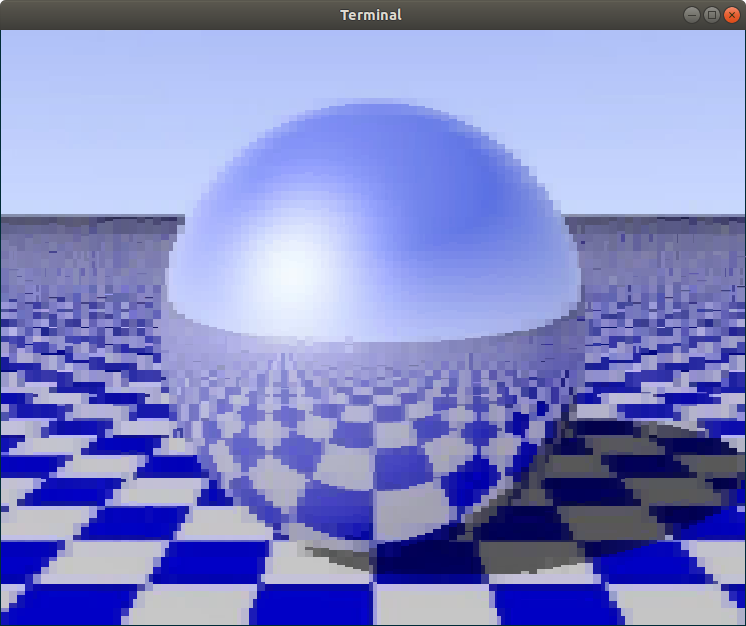
\includegraphics[width=\textwidth]{resources/checker_metal}
  \caption{Example of proposed terminal output}
\end{figure}

\subsection{Rendering Engines and Ray-Tracing}

A rendering engine is an algorithm that takes a scene -- a description of some space with objects -- and generates an image or visual representation of that scene.
There are many different algorithms to do this; in this proposal the recursive ray-tracing algorithm will be discussed and utilized; it was first pioneered by Turner Whitted in his ground-breaking paper {\it An Improved Illumination Model for Shaded Display} \cite{whitted1980improved}.
Ray-tracing was one of the first algorithms developed in the field of computer graphs, and although there have been some improvements since then, the idea behind the algorithm is fairly straight forward.

Ray-tracing revolves around the idea of {\it rays}, a mathematical construct which can be defined by two vectors: an origin point, referred to as $\rayorg$ for some ray $R$, and a direction, referenced as $\raydir$.
These two vectors together represent a ray that starts at the origin and projects along the direction; it is of infinite length. An important addition to the concept of rays is a point along a ray -- this can be defined by using a third variable, which we will call $t$, to represent how far along the ray the point is located.
Therefore, formula \ref{equation:point_on_ray} can be used to get the coordinates of a point in three-dimensional space (assuming $\raydir$ is a unit vector). The mathematics behind ray-tracing are further explored in Section \ref{sec:method}.

\begin{equation}
  \label{equation:point_on_ray}
  \vec{point} = \rayorg + t\raydir
\end{equation}

In ray-tracing, rays are used to simulate the path that light takes as it travels around the scene.
When a ray intersects with an object in the scene, {\it bounce} rays of varying types such reflection, refraction, and shadow can be generated with different directions to simulate how light may travel under different conditions.
It is worth noting that a base assumption is made in ray-tracing when using straight rays as described here: light follows a straight line without changes.
This is only the case in reality when light travels through a vacuum with no gravitational bodies; thus basic ray-tracing is not exactly photorealistic, and does not model phenomena such as atmospheric scattering.

The start of a ray-tracing render is fairly straight forward.


% refactor above and continue writing thread two

\section{Related Work}
\label{sec:relatedwork}

% Summarize the previously published papers and books that are related to your
% proposed research. Whenever possible, you should compare and contrast your
% approach with the ones that have been discussed in the past. As you describe
% related papers, please make sure that you cite them
% properly~\cite{conrad-gecco-selection-study}.

To create an image, a ray-tracer first generates {\it eye-rays}, one for each pixel to render.
These rays have their origin at the camera, and a direction which causes the ray to pass through the pixel to render.
Each ray is then tested against all objects in the scene for intersection, and the intersection with the closest distance is chosen.
This was the only thing the original ray-traced shading algorithm \cite{appel1968some} did, after which the amount of illuminance incident on the point the ray hit, along with some information available from other algorithms (such as if the surface faced a light), dictated the level of darkness of that pixel.

% rewrite above (use stuff on doc) and continue thread three

\section{Method of Approach}
\label{sec:method}

% Use technical diagrams, equations, algorithms, and paragraphs of text to
% describe the research that you intend to complete. See the \LaTeX\ source file
% for the proposal to learn how Figure~\ref{intro-fig1} and Table~\ref{intro-tab1}
% were included. Be sure to number all figures and tables and to explicitly refer
% to them in your text.

\subsection{Ray-Surface Intersection}

Scenes that can be ray-traced must be a collection of surfaces that are mathematically intersectable with a ray.
Any surface that can be defined by $f(\vec{p}) = 0$, that is, $f(\vec{p})$ is $0$ when $\vec{p}$ is on the surface, is intersectable with a ray.
The point of intersection can be found by solving equation \ref{equation:ray_surface_intersection} for $t$ and then using formula \ref{equation:point_on_ray} to calculate the coordinates of that point on the ray.

\begin{equation}
  \label{equation:ray_surface_intersection}
  f(\rayorg + t\raydir) = 0
\end{equation}

In \name, the only surfaces that will be supported are spheres, triangles, and infinite planes, since their surface definition functions are mathematically simple.
For spheres, the surface definition function is function \ref{equation:sphere_surface}, with $S$ representing the sphere.
The intersection point between a ray and a sphere is given by solving equation \ref{equation:ray_sphere_intersection} for $t$ and then using formula \ref{equation:point_on_ray}.
Notice that equation \ref{equation:ray_sphere_intersection} is quadratic, and the number (and values) of the roots give us the $t$ we want to use. The smallest root greater than zero corresponds to the point on the ray which first intersected the sphere. If there are no real roots, then the ray does not intersect the sphere.

\begin{equation}
  \label{equation:sphere_surface}
  f(\vec{p}) = (\vec{p} - \vec{S_{center}})^2 - {S_{radius}}^2
\end{equation}

\begin{equation}
  \label{equation:ray_sphere_intersection}
  (\raydir^2)t^2 + 2(\raydir \cdot (\rayorg - \vec{S_{center}}))t + (\rayorg - \vec{S_{center}})^2 - {S_{radius}}^2 = 0
\end{equation}

For planes, the surface definition function is function \ref{equation:plane_surface}, with $P$ representing the plane.
The plane's {\it offset} is a point on the plane, and the plane's {\it normal} is a vector perpendicular to the plane.
The intersection point between a ray and a plane is given by solving equation \ref{equation:ray_plane_intersection} for $t$ and then using formula \ref{equation:point_on_ray}.

\begin{equation}
  \label{equation:plane_surface}
  f(\vec{p}) = (\vec{p} - \vec{o}) \cdot \vec{n}
\end{equation}

\begin{equation}
  \label{equation:ray_plane_intersection}
  (\vec{P_{normal}} \cdot \raydir)t + \vec{P_{normal}} \cdot (\rayorg - \vec{P_{offset}}) = 0
\end{equation}

For triangles, the intersection is a bit more complicated. First, intersection is tested with the plane the polygon lies in -- that results in some intersection point $Q$. Then,

  % continue writing thread four

\section{Evaluation Strategy}
\label{sec:evaluate}

% Explain what steps you will take to evaluate your proposed method. If you intend
% to conduct experiments, then you must clearly define your evaluation metrics.

\section{Research Schedule}
\label{sec:schedule}

% Identify the main phases and tasks of your research project and set deadlines
% for when you will be able to complete each of these items.

\section{Conclusion}
\label{sec:conclusion}

% Provide a summary of your proposed research and suggest the impact that it may
% have on the discipline of computer science. If possible, you may also suggest
% some areas for future research.

\bibliographystyle{plain}
\bibliography{senior_thesis_proposal}
\end{document}
